\section{原始视频、时间轴与输入条件}
\label{sec:input}
完整pipeline首先确定每个观测对应哪个采集、相机、帧和物理坐标，再进入手部与物体分支。视频切分阶段输出短片及索引，记录来源视频、起止时间、实际帧数与帧率。需要精确边界时重新编码，避免仅按压缩流关键帧切割引入偏移。多相机和同一长视频的不同切片按采集ID分组，训练／验证／测试划分在滑窗之前固定。

第一视角主线保留标注版视频的原生时间戳与相机参数。Raw版与标注版并不保证同一帧号对应同一时刻，必须通过实际长度与时间轴核对。图预测使用32帧历史和至少1秒的未来目标；这与制作视频时使用3fps或10fps回放是不同概念。

系统保留两种可追溯的感知输入条件：EgoDemo线路使用官方手姿态、同采集双目和派生物体几何；独立RGB-D验证线路使用MediaPipe与FoundationPose真实推理。后者用于验证感知模块能运行、可输出什么以及耗时多少，不能直接替代前者的预测测试结果。输入无深度、无尺度或无物体模型时，也不能把另一个RGB-D场景的假设自动转移过去。

\section{手部姿态估计与坐标对齐}
\label{sec:hands}
\subsection{从图像到双手21点}
在线分支采用MediaPipe Hands的两阶段设计：先定位手掌区域，再回归手部关键点\cite{zhang2020mediapipe}。项目封装按帧返回左右手各21点和有效性信息，保留腕部、四指关节与拇指拓扑。未检测到的整只手与置信字段保持NaN，由下游mask明确排除。对非镜像输入按后端自拍约定交换左右手标签；不通过水平翻转原图来掩盖身份错误。

图像输出$(x,y,z_{rel})$中的$x,y$按图像尺寸归一化，$z_{rel}$是腕部相对深度，并非米制相机坐标。左右手分类分数也不是关节定位精度。实时分支和训练数据分支都保留这些语义，避免下游将两个不同坐标空间的量直接相减。

\begin{figure}[H]
\centering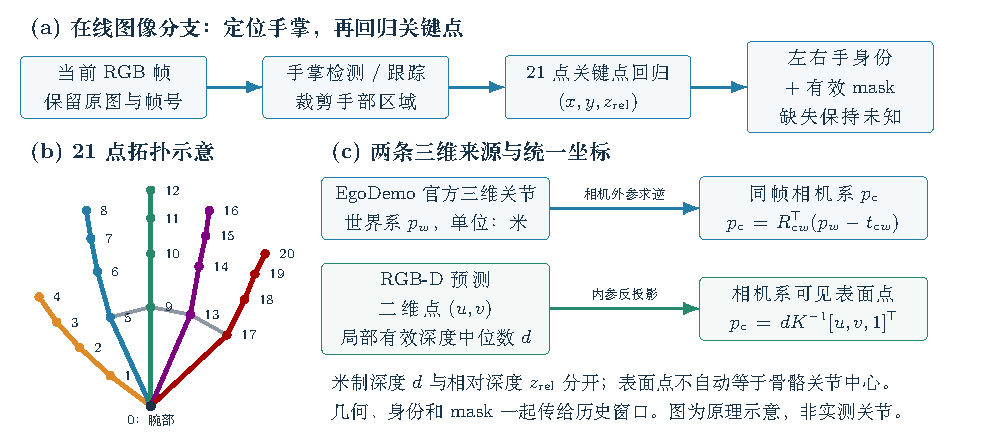
\includegraphics[width=\textwidth]{figures/hand_pose_principle.pdf}
\caption{手部姿态原理图。上：手掌定位到21点回归的在线分支。左下：腕部与五指的21点拓扑。右下：官方世界系关节经相机外参转换，以及RGB-D二维关键点经深度反投影，两条来源分开表达。所有点与模块均为原理示意；真实演示见图\ref{fig:handcoords}和图\ref{fig:rgbdhuman}。}
\label{fig:handprinciple}
\end{figure}

\subsection{官方三维姿态与RGB-D表面提升}
EgoDemo线路读取官方世界坐标手关节和同帧相机到世界变换。若$T_{cw}=[R_{cw},t_{cw}]$表示相机到世界，则
\begin{equation}
 p_c=R_{cw}^{\mathsf T}(p_w-t_{cw}),\qquad
 u=\pi(Kp_c).
\end{equation}
针孔投影$\pi$将齐次坐标除以正深度；负深度、图外点、缺失关节分别保留标记。后续时序特征还会将历史关节转换到锚点相机系，降低头部运动造成的坐标变化。图\ref{fig:handcoords}给出真实视频上的双手叠加和多视角坐标诊断。

\begin{figure}[H]
\centering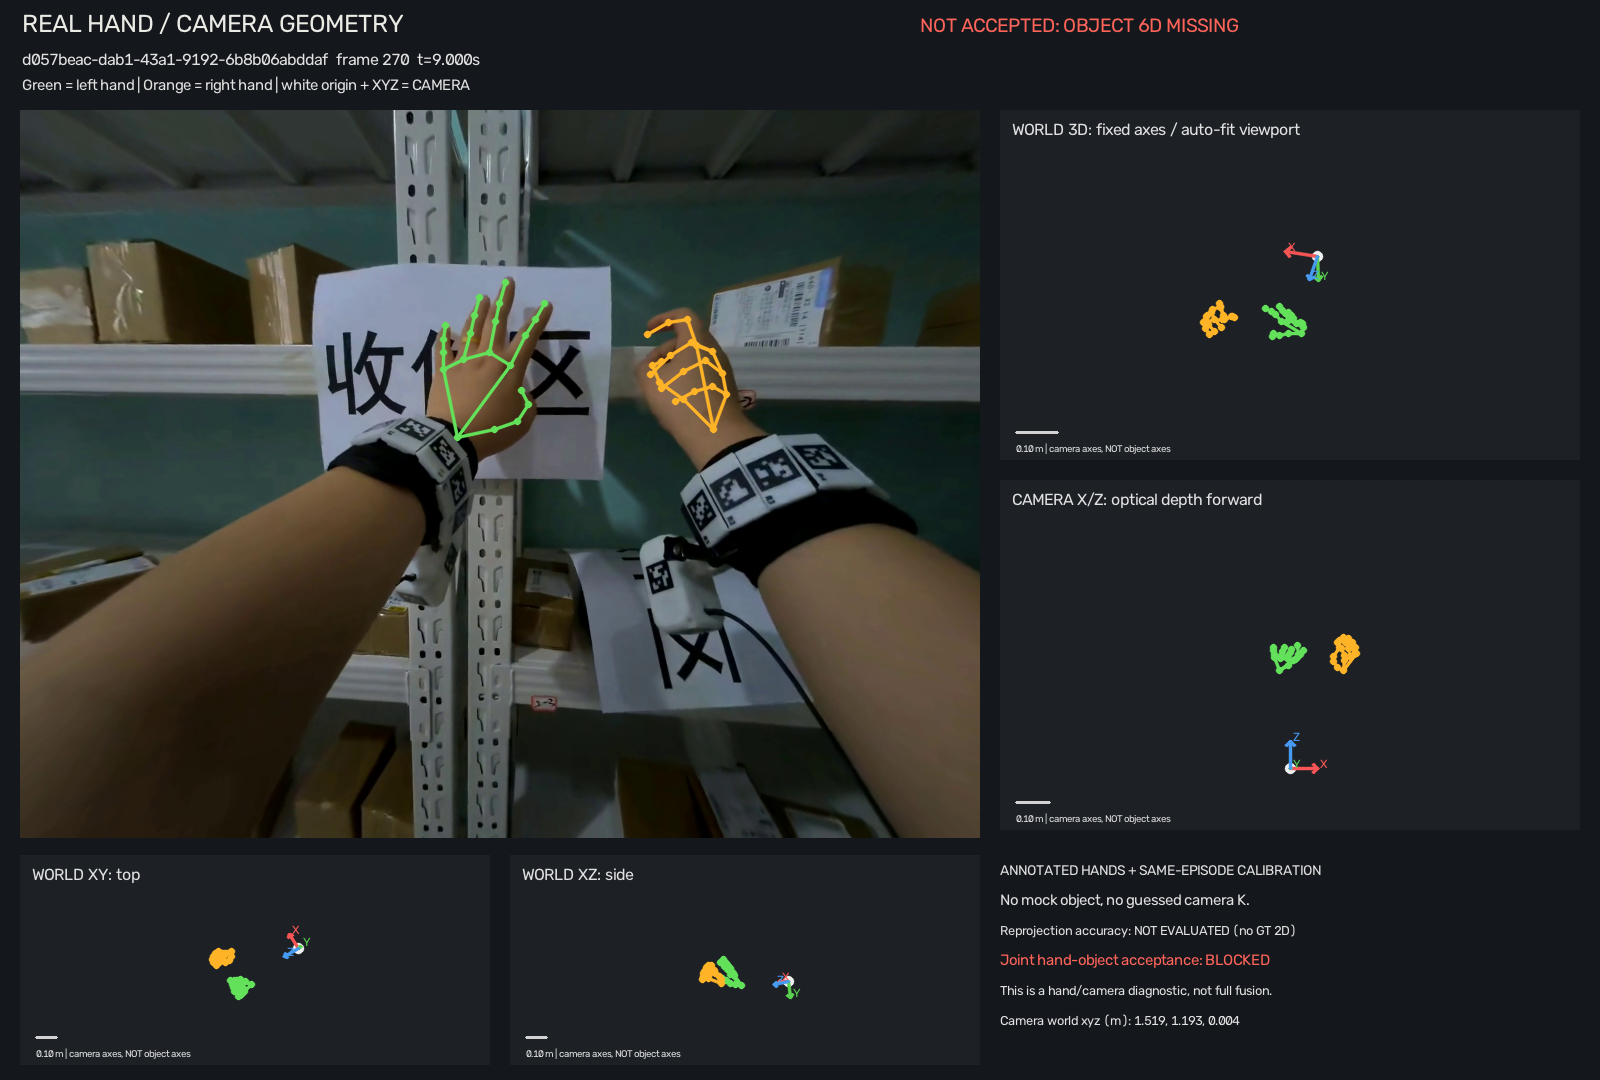
\includegraphics[width=.74\textwidth]{figures/hand_ego_coordinates.png}
\caption{第一视角手部姿态与相机／世界坐标演示。左侧为来源手关节投影，右侧与下侧为不同坐标视图；并非MediaPipe检测结果。该原图来自10月22日手／相机专项检查，画面中的物体缺失提示属于当时的阶段状态，不代表后续物体几何仍未构建。保留原图文字以维持来源可追溯。}
\label{fig:handcoords}
\end{figure}

对有对齐深度的RGB-D输入，可在预测二维关键点附近取有效深度中位数$d$，反投影为
\begin{equation}
 p_c=dK^{-1}[u,v,1]^{\mathsf T}.
\end{equation}
HO-Cap实现使用半径2像素邻域，至少3个有效深度，并限制10\%--90\%分位跨度不超过0.04米。遮挡边缘深度混杂时拒绝提升。这个点表示二维关节射线对应的可见表面，不能自动视为真实骨骼关节的三维中心。

\subsection{真实同帧手物演示}
图\ref{fig:rgbdhuman}左侧展示DexYCB真人持碗的手部预测与物体位姿同时输出；右侧展示HO-Cap四个物体的独立位姿跟踪。它们验证真实模块之间的输入输出衔接，分别保留各自场景和输入条件。工程实现可将手部CPU推理与物体GPU推理并行执行，按同一帧号等待结果齐全后再渲染。

\begin{figure}[H]
\centering
\begin{minipage}{.48\textwidth}\centering
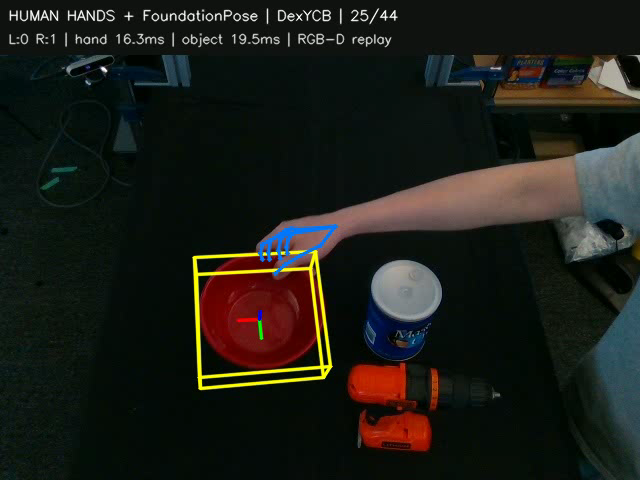
\includegraphics[width=\linewidth]{figures/hand_object_rgbd.png}\\\small (a) DexYCB：21点手骨架、物体框和XYZ轴
\end{minipage}\hfill
\begin{minipage}{.48\textwidth}\centering
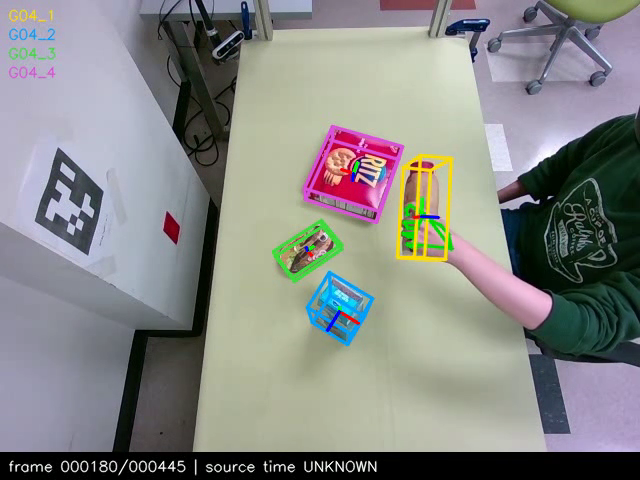
\includegraphics[width=\linewidth]{figures/hocap_four_objects_f180.png}\\\small (b) HO-Cap：同一人手场景中的四物体6D
\end{minipage}
\caption{两条真实RGB-D感知演示，均为既有输出。左图蓝色手骨架来自模型预测；右图从446帧完整视频的第180帧直接解码。颜色区分物体身份，坐标轴表示估计姿态。不同场景不拼接成一次运行；同帧叠加不自动证明手关节与物体已完成独立米制精度验收。}
\label{fig:rgbdhuman}
\end{figure}

\section{物体6D位姿与表面运动建模}
\label{sec:pose6d}
\subsection{六自由度与刚体变换}
6D位姿由平移三自由度和旋转三自由度组成。用物体到相机的齐次变换表示为
\begin{equation}
 T_{oc}=\begin{bmatrix}R&t\\0&1\end{bmatrix},\quad
 R^{\mathsf T}R=I,\quad\det R=1,
\end{equation}
物体模型点$x_o$经$x_c=Rx_o+t$变换后投影到图像。相机运动存在时，用$T_{ow}=T_{cw}T_{oc}$统一到世界系。后续特征中使用旋转矩阵前两列的六维编码；“旋转六维编码”和“物体六自由度位姿”是两个不同概念。

\subsection{RGB-D、mesh与FoundationPose分支}
已知几何模型的RGB-D分支采用FoundationPose\cite{wen2024foundationpose}。注册时输入当前RGB、米制深度、相机内参、目标mask和对应mesh；从姿态候选出发进行学习式细化与评分，随后使用前帧状态和当前RGB-D连续跟踪。项目使用真实scorer／refiner权重，保留原始mesh坐标和返回的物体到相机变换。初始mask与物体匹配，后续跟踪不读取未来位姿参考。

该分支的关键工程约束是单位与物体身份：uint16毫米深度乘0.001后与mesh统一为米；网格不能任意换模型、改尺度或重心而不记录变换。碗等对称物体的朝向可能存在等价解，单看框贴合不能证明全部旋转角精确。图\ref{fig:posecloud}展示预测mesh、估计坐标轴与真实深度点云处于同一相机系的具体输出。

\begin{figure}[H]
\centering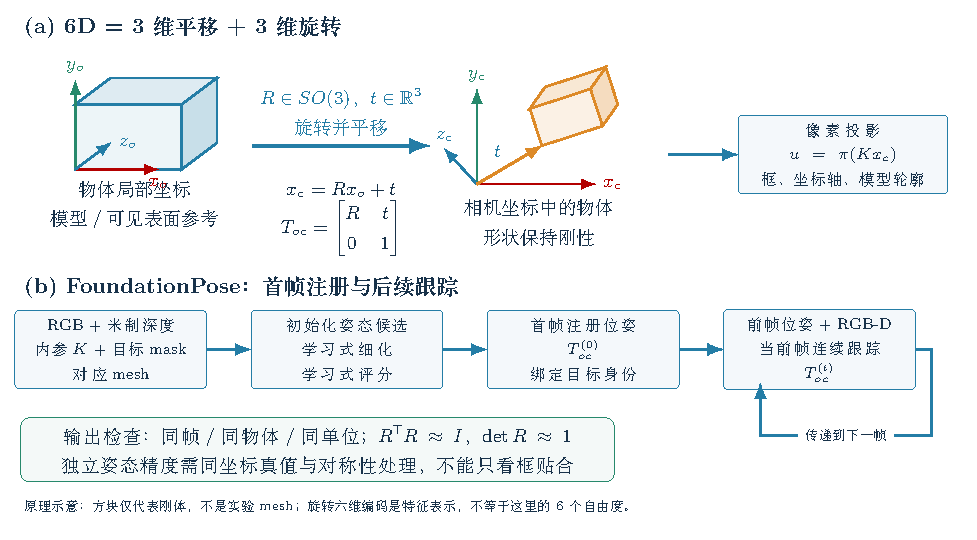
\includegraphics[width=\textwidth]{figures/pose6d_principle.pdf}
\caption{物体6D与FoundationPose原理图。上：物体点由旋转$R$和平移$t$变换到相机系，经内参投影为框、轴或轮廓。下：首帧RGB-D、mask与mesh用于姿态候选细化和评分，后续由前帧位姿与当前观测连续跟踪。图中方块是几何示意，不是实测模型；真实点云与mesh输出见图\ref{fig:posecloud}。}
\label{fig:poseprinciple}
\end{figure}

\begin{figure}[H]
\centering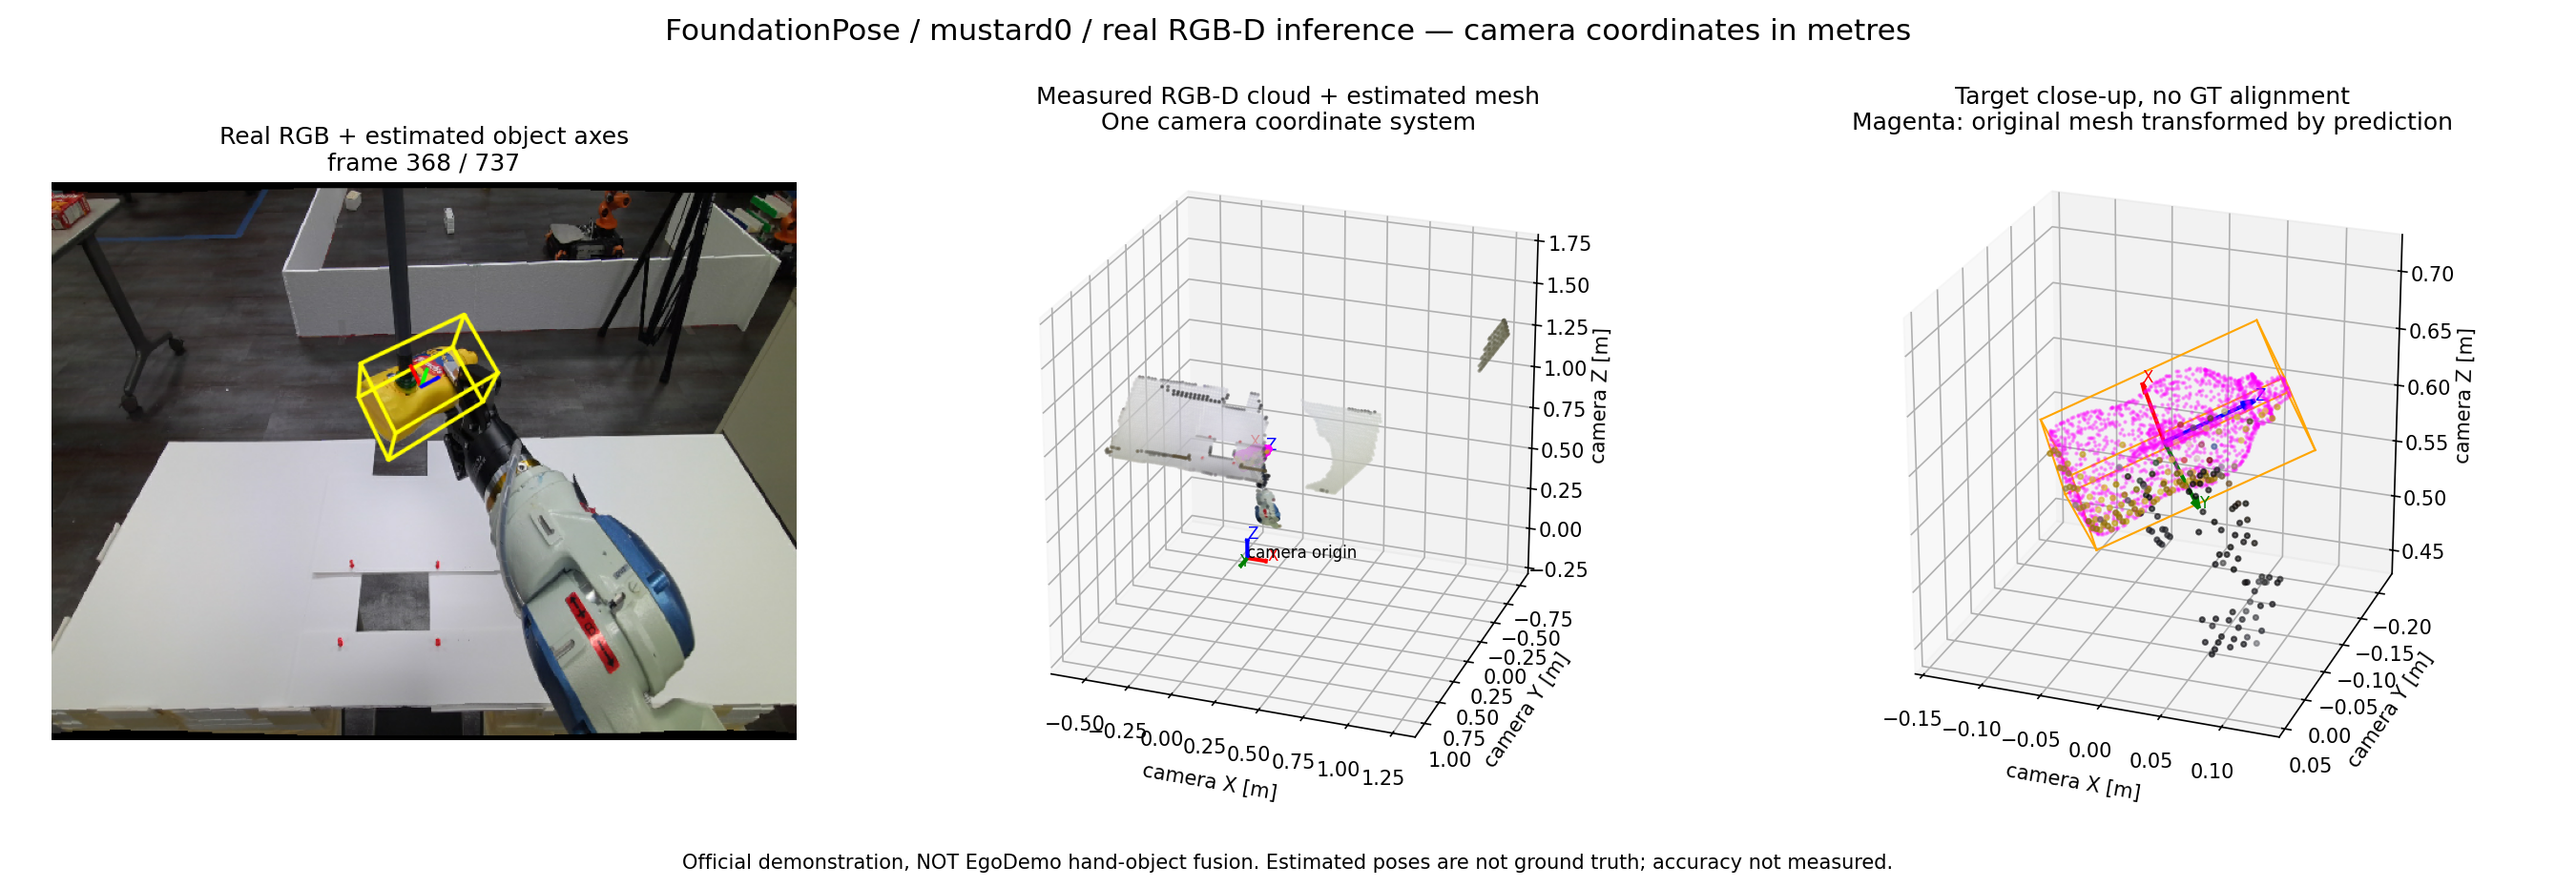
\includegraphics[width=\textwidth]{figures/pose6d_pointcloud.png}
\caption{FoundationPose独立后端验证：RGB叠加、真实深度反投影点云及预测mesh局部图。紫色mesh由估计位姿变换，不按GT重新对齐。这个737帧公开样例包含机械臂，仅用于说明6D后端与三维坐标计算；真人手物演示见图\ref{fig:rgbdhuman}，第一视角主线见图\ref{fig:handcoords}和图\ref{fig:surface}.}
\label{fig:posecloud}
\end{figure}

\subsection{EgoDemo双目重建与无CAD几何分支}
第一视角物体通常没有逐个可用的CAD模型，实际工程使用同采集双目、实例表面种子和跨帧点对应来构建局部参考系。相机相对变换为$T_{lr}=T_{rw}^{-1}T_{lw}$。先检查标定与像素对应的一致性，再校正双目、估计视差并进行左右一致性筛选；校正后的理想情形满足$Z=f_xb/d$，非校正情形用双投影矩阵三角化。来源中存在标定修正与留出像素检查，修正记录与原参数同时保留。

连续轨迹提供对应点$\{a_j,b_j\}$，刚性估计求解
\begin{equation}
 (R^*,t^*)=\arg\min_{R\in SO(3),t}\sum_{j\in\mathcal I}
 \|Ra_j+t-b_j\|_2^2 .
\end{equation}
实现用RANSAC剔除错误对应，再对中心化协方差做SVD求$R,t$。本地默认要求至少8个内点、内点比例至少0.65、距离阈值0.012米；同时检查点云跨度与第二奇异值，避免近点状／线状目标的旋转不可观。另有稀疏参考点到后续图像的PnP分支，保留重投影残差与内点数。

物体局部原点来自初始可见表面，轴可由初始相机定义，未必等于CAD中心或语义轴。关联相同名字不代表坐标系已经对齐：跨tracklet拼接还需相对刚体变换和表面一致性证据。纸张、布料等非刚体保留点轨迹或局部表面参考系，铰接工具按部件表达；它们不强制拟合为整物体刚体。

\begin{figure}[H]
\centering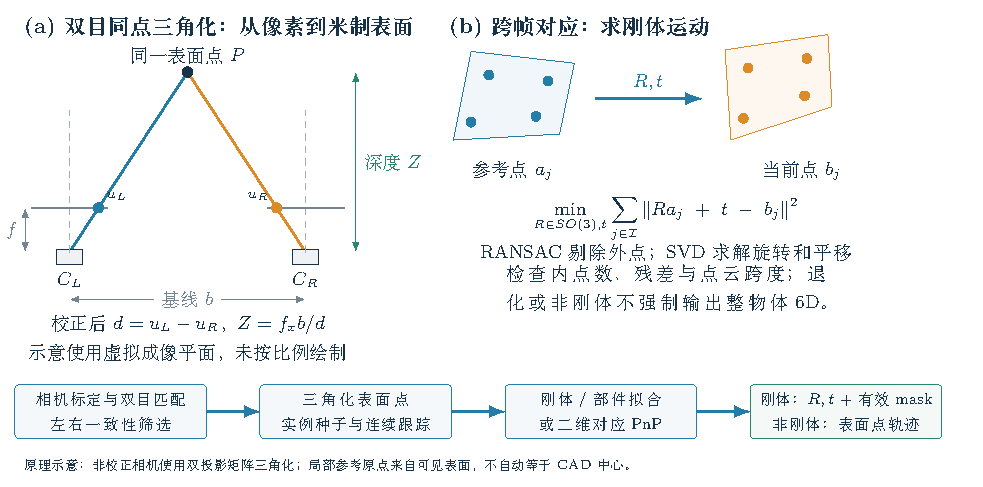
\includegraphics[width=\textwidth]{figures/stereo_geometry_principle.pdf}
\caption{双目重建与跨帧刚体拟合原理图。左上：同一表面点由左右像素射线交会恢复深度，理想校正情形为$Z=f_xb/d$。右上：参考帧与当前帧的对应点，经RANSAC筛选后用SVD求刚体变换。下：从标定、点匹配到局部几何输出的工程路径。相机和点集为原理示意，真实表面种子见图\ref{fig:surface}。}
\label{fig:stereoprinciple}
\end{figure}

\begin{figure}[H]
\centering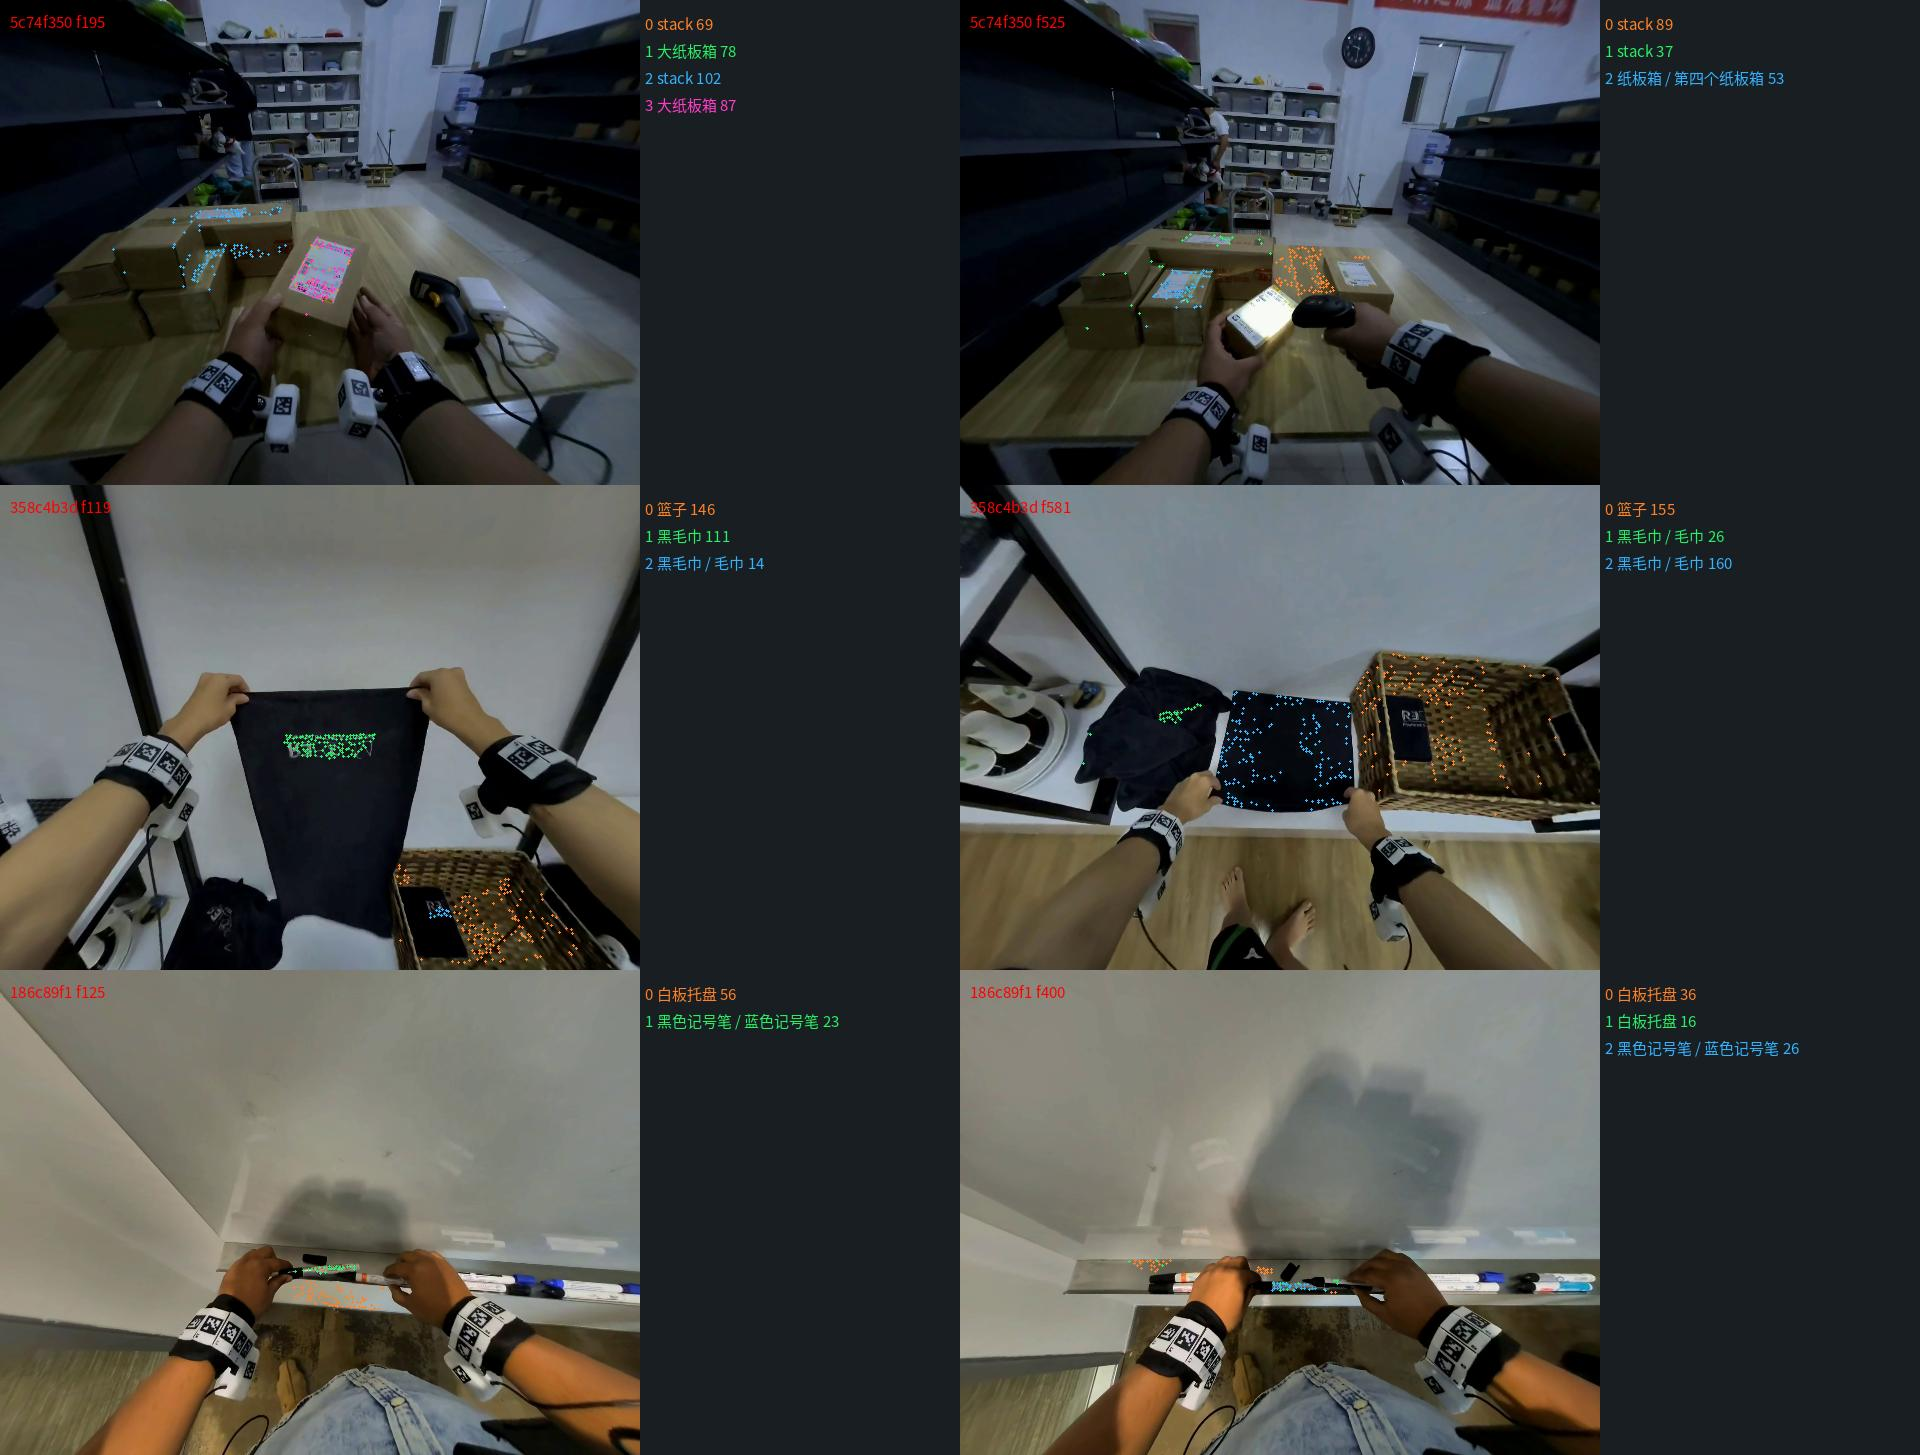
\includegraphics[width=.64\textwidth]{figures/egodemo_surface_seeds.jpg}
\caption{EgoDemo第一视角的真实表面种子与点分布示例，包含纸盒、织物和托盘／笔等不同目标。图为已保存的候选几何准备结果，数字表示相应实例的点数，不能解释为姿态准确率。该分支为后续跨帧跟踪、刚体／部件拟合和非刚体表面描述提供观测。}
\label{fig:surface}
\end{figure}

\section{感知模块的指标与验证图}
\label{sec:perceptionmetrics}
\subsection{按指标回答不同问题}
感知验证按输入对齐、输出覆盖、几何一致性、运行时延和独立精度分别报告。覆盖率回答“有多少帧输出有效值”；几何一致性回答“变换、投影与文件是否自洽”；独立精度回答“与外部真值相差多少”。只有具备同物体、同帧、同坐标的独立参考，才能计算位置误差$e_t=\|\hat t-t^*\|_2$及旋转误差
\begin{equation}
 e_R=\arccos\!\left(\operatorname{clip}_{[-1,1]}\!\left(\frac{\operatorname{tr}(\hat RR^{*\mathsf T})-1}{2}\right)\right).
\end{equation}
式中clip限制输入到$[-1,1]$；对称物体需按对称等价类定义评价。手部三维精度可用MPJPE或带阈值的PCK，二维可用独立关键点重投影误差。现有感知材料没有提供完整独立精度评测，因此这些项写为未测，不用覆盖率或轨迹变化替代。

\begin{table}[H]
\centering\small\setlength{\tabcolsep}{5pt}
\resizebox{\textwidth}{!}{\begin{tabular}{llll}
\toprule 环节／验证集 & 已测结果 & 分母与范围 & 结果含义\\\midrule
EgoDemo双手来源检查 & 双手同时有效7146/7164 & 两采集1194+5970帧 & 来源姿态覆盖，非检测精度\\
EgoDemo标定像素复核 & 275直接一致，20修正后检查 & 300采集；另4待复核、1不一致 & 抽样像素一致性\\
FoundationPose后端 & 737/737有限合法刚体输出 & 独立公开RGB-D样例 & 运行覆盖与数值合法性\\
DexYCB手物联合输出 & 44/44右手与物体均有输出 & 同一44帧，三次复测 & 模块联调与短片覆盖\\
HO-Cap多物体输出 & 446帧；四物体各446有效 & 真人单采集；手任一有效446帧 & 多目标工程覆盖\\
感知独立位置／旋转／手精度 & 未测 & 独立参考尚未形成对应结果 & 不报告虚构准确率\\
\bottomrule
\end{tabular}}
\caption{感知验证结果与统计口径，来自既有运行JSON／NPZ／CSV。不同数据集的计数不相加成为统一测试集。具体失败和缺失状态按各次运行保留，而非覆盖成一个总通过率。}
\label{tab:perception}
\end{table}

\begin{figure}[H]
\centering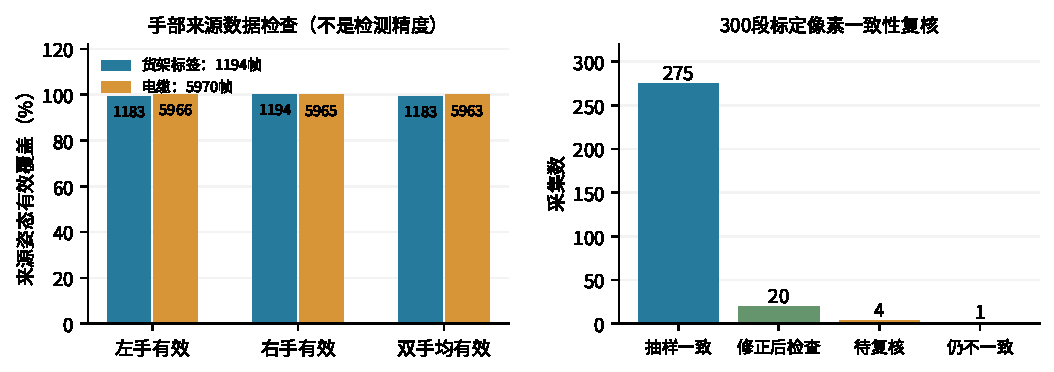
\includegraphics[width=\textwidth]{figures/hand_calibration_coverage.pdf}
\caption{手部来源覆盖与相机像素一致性验证图。左侧柱顶为有效帧数、柱高为对应采集中的比例；右侧为300段重建流程最终汇总中的标定状态。两者分别验证数据可用性与几何输入，不是学习模型精度。}
\label{fig:coverage}
\end{figure}

\subsection{6D数值验证与逐帧延迟}
图\ref{fig:perceptionvalidation}直接从737个保存位姿和44帧联合输出的CSV复算。旋转正交性最大元素偏差为$3.472\times10^{-6}$，$|\det R-1|$最大约$1.594\times10^{-6}$；说明输出满足刚体矩阵数值约束。平移轨迹展示实际运动，不是相对于真值的误差曲线。

\begin{figure}[H]
\centering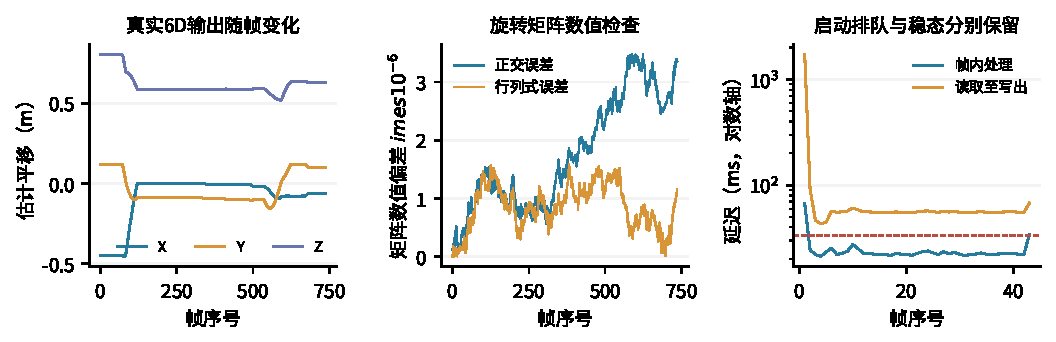
\includegraphics[width=\textwidth]{figures/perception_validation.pdf}
\caption{逐帧感知验证。左：6D输出的平移变化；中：旋转正交性与行列式偏差；右：DexYCB最终复测中除注册帧外的帧内处理和读取至写出时延。右图采用对数轴保留首个预取帧跨注册阶段的排队峰值，未裁掉慢帧。矩阵误差属于数值检查，不属于姿态真值误差。}
\label{fig:perceptionvalidation}
\end{figure}

\subsection{感知性能优化与实际边界}
同一44帧DexYCB片段在L40上比较不同手模型、物体跟踪迭代和输入预取。最终lite手模型、一次物体跟踪、CPU／GPU同帧并行、有界预取的三次复测稳态处理能力为41.409、41.471、41.524 FPS；帧内P95为27.056、27.967、27.265ms。图\ref{fig:runtime}保留较慢配置，说明优化的实际变化。

\begin{figure}[H]
\centering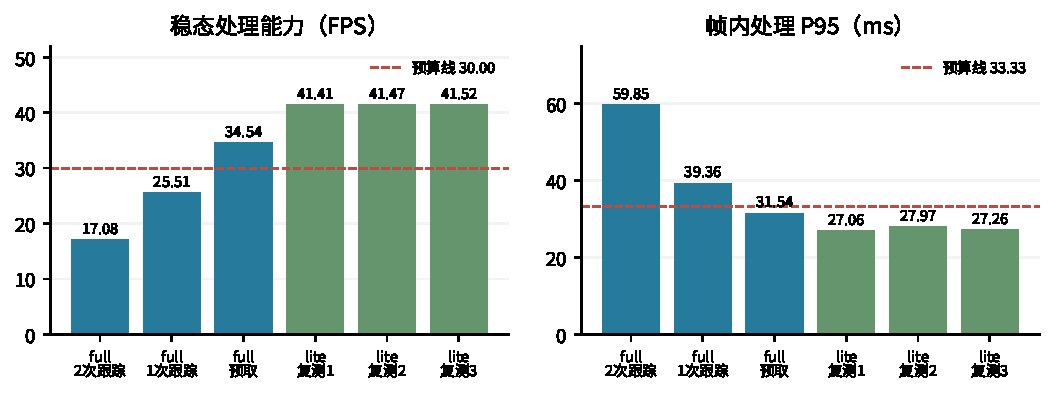
\includegraphics[width=\textwidth]{figures/perception_runtime.pdf}
\caption{真实感知配置的吞吐与帧内P95，均来自同一44帧片段，稳态分母为除注册帧外的43帧。虚线对应30FPS处理预算。改手模型和跟踪迭代数可能影响精度，图中只报告实测性能；三次复测不是132个独立样本。}
\label{fig:runtime}
\end{figure}

最终三轮各有2/43帧超过33.33ms，首帧注册约1.63--1.66秒，读取至写出P95为55.49--66.90ms。因此可以报告短序列稳态处理能力，不能把MP4的30FPS或环路时延写成相机曝光到屏幕显示的硬实时指标。HO-Cap四物体配置的稳态约6.87FPS，单独记录其多物体计算量与输入条件，不套用单碗场景的速度。
